\documentclass[a4paper, 14pt]{extarticle}

% Поля
%--------------------------------------
\usepackage{geometry}
\geometry{a4paper,tmargin=2cm,bmargin=2cm,lmargin=3cm,rmargin=1cm}
%--------------------------------------


%Russian-specific packages
%--------------------------------------
\usepackage[T2A]{fontenc}
\usepackage[utf8]{inputenc} 
\usepackage[english, main=russian]{babel}
%--------------------------------------

\usepackage{textcomp}

% Красная строка
%--------------------------------------
\usepackage{indentfirst}               
%--------------------------------------             


%Graphics
%--------------------------------------
\usepackage{graphicx}
\graphicspath{ {./images/} }
\usepackage{wrapfig}
%--------------------------------------

% Полуторный интервал
%--------------------------------------
\linespread{1.3}                    
%--------------------------------------

%Выравнивание и переносы
%--------------------------------------
% Избавляемся от переполнений
\sloppy
% Запрещаем разрыв страницы после первой строки абзаца
\clubpenalty=10000
% Запрещаем разрыв страницы после последней строки абзаца
\widowpenalty=10000
%--------------------------------------

%Списки
\usepackage{enumitem}

%Подписи
\usepackage{caption} 

%Гиперссылки
\usepackage{hyperref}

\hypersetup {
	unicode=true
}

%Рисунки
%--------------------------------------
\DeclareCaptionLabelSeparator*{emdash}{~--- }
\captionsetup[figure]{labelsep=emdash,font=onehalfspacing,position=bottom}
%--------------------------------------

\usepackage{tempora}

%Листинги
%--------------------------------------
\usepackage{listings}
\lstset{
  basicstyle=\ttfamily\footnotesize, 
  %basicstyle=\footnotesize\AnkaCoder,        % the size of the fonts that are used for the code
  breakatwhitespace=false,         % sets if automatic breaks shoulbd only happen at whitespace
  breaklines=true,                 % sets automatic line breaking
  captionpos=t,                    % sets the caption-position to bottom
  inputencoding=utf8,
  frame=single,                    % adds a frame around the code
  keepspaces=true,                 % keeps spaces in text, useful for keeping indentation of code (possibly needs columns=flexible)
  keywordstyle=\bf,       % keyword style
  numbers=left,                    % where to put the line-numbers; possible values are (none, left, right)
  numbersep=5pt,                   % how far the line-numbers are from the code
  xleftmargin=25pt,
  xrightmargin=25pt,
  showspaces=false,                % show spaces everywhere adding particular underscores; it overrides 'showstringspaces'
  showstringspaces=false,          % underline spaces within strings only
  showtabs=false,                  % show tabs within strings adding particular underscores
  stepnumber=1,                    % the step between two line-numbers. If it's 1, each line will be numbered
  tabsize=2,                       % sets default tabsize to 8 spaces
  title=\lstname                   % show the filename of files included with \lstinputlisting; also try caption instead of title
}
%--------------------------------------

%%% Математические пакеты %%%
%--------------------------------------
\usepackage{amsthm,amsfonts,amsmath,amssymb,amscd}  % Математические дополнения от AMS
\usepackage{mathtools}                              % Добавляет окружение multlined
\usepackage[perpage]{footmisc}
%--------------------------------------

%--------------------------------------
%			НАЧАЛО ДОКУМЕНТА
%--------------------------------------

\begin{document}

%--------------------------------------
%			ТИТУЛЬНЫЙ ЛИСТ
%--------------------------------------
\begin{titlepage}
\thispagestyle{empty}
\newpage


%Шапка титульного листа
%--------------------------------------
\vspace*{-60pt}
\hspace{-65pt}
\begin{minipage}{0.3\textwidth}
\hspace*{-20pt}\centering

\includegraphics[width=\textwidth]{emblem}
\end{minipage}
\begin{minipage}{0.67\textwidth}\small \textbf{
\vspace*{-0.7ex}
\hspace*{-6pt}\centerline{Министерство науки и высшего образования Российской Федерации}
\vspace*{-0.7ex}
\centerline{Федеральное государственное бюджетное образовательное учреждение }
\vspace*{-0.7ex}
\centerline{высшего образования}
\vspace*{-0.7ex}
\centerline{<<Московский государственный технический университет}
\vspace*{-0.7ex}
\centerline{имени Н.Э. Баумана}
\vspace*{-0.7ex}
\centerline{(национальный исследовательский университет)>>}
\vspace*{-0.7ex}
\centerline{(МГТУ им. Н.Э. Баумана)}}
\end{minipage}
%--------------------------------------

%Полосы
%--------------------------------------
\vspace{-25pt}
\hspace{-35pt}\rule{\textwidth}{2.3pt}

\vspace*{-20.3pt}
\hspace{-35pt}\rule{\textwidth}{0.4pt}
%--------------------------------------

\vspace{1.5ex}
\hspace{-35pt} \noindent \small ФАКУЛЬТЕТ\hspace{80pt} <<Информатика и системы управления>>

\vspace*{-16pt}
\hspace{47pt}\rule{0.83\textwidth}{0.4pt}

\vspace{0.5ex}
\hspace{-35pt} \noindent \small КАФЕДРА\hspace{50pt} <<Теоретическая информатика и компьютерные технологии>>

\vspace*{-16pt}
\hspace{30pt}\rule{0.866\textwidth}{0.4pt}
  
\vspace{11em}

\begin{center}
\Large {\bf Лабораторная работа № 2} \\
\large {\bf по курсу <<Теория искусственных нейронных сетей>>} \\
\large <<Разработка многослойного персептрона на основе обратного распространения ошибки FFNN>>
\end{center}\normalsize

\vspace{8em}


\begin{flushright}
  {Студентка группы ИУ9-72Б Самохвалова П. С. \hspace*{15pt}\\
  \vspace{2ex}
  Преподаватель Каганов Ю. Т.\hspace*{15pt}}
\end{flushright}

\bigskip

\vfill
 

\begin{center}
\textsl{Москва 2023}
\end{center}
\end{titlepage}
%--------------------------------------
%		КОНЕЦ ТИТУЛЬНОГО ЛИСТА
%--------------------------------------

\renewcommand{\ttdefault}{pcr}

\setlength{\tabcolsep}{3pt}
\newpage
\setcounter{page}{2}

\section{Цель работы}\label{Sect::goal}

Изучение многослойного персептрона, исследование его работы на основе использования различных методов оптимизации и целевых функций.

\section{Задание}\label{Sect::task}

\begin{itemize}
    \item Реализовать на языке высокого уровня многослойный персептрон и проверить его работоспособность на примере данных, выбранных из MNIST dataset.
    \item Исследовать работу персептрона на основе использования различных целевых функций. (среднеквадратичная ошибка, перекрестная энтропия, дивергенция Кульбака-Лейблера).
    \item Исследовать работу многослойного персептрона с использованием различных методов оптимизации (градиентный, Флетчера-Ривза (FR), Бройдена-Флетчера-Гольдфарба-Шенно (BFGS)).
    \item Подготовить отчет с распечаткой текста программы, графиками результатов исследования и анализом результатов.
\end{itemize}

\section{Практическая реализация}\label{Sect::code}

Исходный код программы представлен в листинге~\ref{lst:code1}.

\begin{lstlisting}[language={python},caption={Многослойный персептрон},label={lst:code1}]
import random
import pickle
import gzip
import numpy as np
from matplotlib import pyplot as plt


def load_data():
    with gzip.open('../data/mnist.pkl.gz', 'rb') as f:
        (training_data, validation_data, test_data) = pickle.load(f, encoding='latin1')
    return (training_data, validation_data, test_data)


def load_data_wrapper():
    tr_d, va_d, te_d = load_data()
    training_inputs = [np.reshape(x, (784, 1)) for x in tr_d[0]]
    training_results = [vectorized_result(y) for y in tr_d[1]]
    training_data = list(zip(training_inputs, training_results))
    validation_inputs = [np.reshape(x, (784, 1)) for x in va_d[0]]
    validation_data = list(zip(validation_inputs, va_d[1]))
    test_inputs = [np.reshape(x, (784, 1)) for x in te_d[0]]
    test_data = list(zip(test_inputs, te_d[1]))
    return (training_data, validation_data, test_data)


def vectorized_result(j):
    e = np.zeros((10, 1))
    e[j] = 1.0
    return e


def sigmoid(x):
    return 1 / (1 + np.exp(-x))


def sigmoid_der(x):
    return sigmoid(x) * (1 - sigmoid(x))


def relu(x):
    x = x.flatten()
    return np.array([[max(c, 0)] for c in x])


def relu_der(x):
    x = x.flatten()
    return np.array([[1 if c > 0 else 0] for c in x])


def softmax(z):
    e_z = np.exp(z - np.max(z))
    return e_z / e_z.sum()


def softmax_der(z):
    s = softmax(z)
    return np.diag(s) - np.outer(s, s)


def mse(y_true, y_received):
    return np.linalg.norm(y_true - y_received)


def mse_der(y_true, y_received):
    return y_true - y_received


def categorical_cross_entropy(y0, y):
    return -(y0 * np.log(y) + (1 - y0) * np.log(1 - y))


def categorical_cross_entropy_der(y0, y):
    return -(y0 / y - (1 - y0) / (1 - y))


def kl_divergence(y0, y):
    if y0 == 0:
        return 0
    else:
        return y0 * np.log(y0 / y)


def kl_divergence_der(y0, y):
    return np.log(y0 / y) + 1


class MultilayerPerceptron(object):

    def __init__(self, sizes, optimization_method, activation_function, loss_function):
        self.num_layers = len(sizes)
        self.optimization_method = optimization_method
        self.activation_function = activation_function
        if activation_function == sigmoid:
            self.activation_function_der = sigmoid_der
        elif activation_function == relu:
            self.activation_function_der = relu_der
        elif activation_function == softmax:
            self.activation_function_der = softmax_der
        self.loss_function = loss_function
        if loss_function == mse:
            self.loss_function_der = mse_der
        elif loss_function == categorical_cross_entropy:
            self.loss_function_der = categorical_cross_entropy_der
        elif self.loss_function == kl_divergence:
            self.loss_function_der = kl_divergence_der
        self.sizes = sizes
        self.biases = [np.random.randn(y, 1) for y in sizes[1:]]
        self.weights = [np.random.randn(y, x) for x, y in zip(sizes[:-1], sizes[1:])]
        self.loss = []

    def feedforward(self, a):
        for b, w in zip(self.biases, self.weights):
            a = self.activation_function(np.dot(w, a) + b)
        return a

    def train(self, training_data, epochs, mini_batch_size, eta, test_data):
        if self.optimization_method == "gradient_descent":
            self.SGD(training_data, epochs, mini_batch_size, eta, test_data)
        elif self.optimization_method == "fletcher_reeves":
            self.fletcher_reeves_optimization(training_data, epochs, mini_batch_size, eta, test_data)
        elif self.optimization_method == "bfgs":
            self.bfgs(training_data, epochs, mini_batch_size, test_data)

    def SGD(self, training_data, epochs, mini_batch_size, eta, test_data):
        n = len(training_data)
        for j in range(epochs):
            random.shuffle(training_data)
            mini_batches = [training_data[k : k+mini_batch_size] for k in range(0, n, mini_batch_size)]
            for mini_batch in mini_batches:
                self.update_mini_batch(mini_batch, eta)
            self.test(test_data)

    def update_mini_batch(self, mini_batch, eta):
        nabla_b = [np.zeros(b.shape) for b in self.biases]
        nabla_w = [np.zeros(w.shape) for w in self.weights]
        for x, y in mini_batch:
            delta_nabla_b, delta_nabla_w = self.backprop(x, y)
            nabla_b = [nb + dnb for nb, dnb in zip(nabla_b, delta_nabla_b)]
            nabla_w = [nw + dnw for nw, dnw in zip(nabla_w, delta_nabla_w)]
        self.weights = [w - (eta / len(mini_batch)) * nw for w, nw in zip(self.weights, nabla_w)]
        self.biases = [b - (eta / len(mini_batch)) * nb for b, nb in zip(self.biases, nabla_b)]

    def backprop(self, x, y):
        nabla_b = [np.zeros(b.shape) for b in self.biases]
        nabla_w = [np.zeros(w.shape) for w in self.weights]

        activation = x
        activations = [x]
        zs = []
        for b, w in zip(self.biases, self.weights):
            z = np.dot(w, activation) + b
            zs.append(z)
            activation = self.activation_function(z)
            activations.append(activation)

        delta = self.loss_function_der(activations[-1], y) * self.activation_function_der(zs[-1])
        nabla_b[-1] = delta
        nabla_w[-1] = np.dot(delta, activations[-2].transpose())

        for l in range(2, self.num_layers):
            z = zs[-l]
            sp = self.activation_function_der(z)
            delta = np.dot(self.weights[-l + 1].transpose(), delta) * sp
            nabla_b[-l] = delta
            nabla_w[-l] = np.dot(delta, activations[-l - 1].transpose())

        return (nabla_b, nabla_w)

    def fletcher_reeves(self, g, old_g, d):
        beta = np.dot(g.T, g) / np.dot(old_g.T, old_g)
        new_d = -g + beta * d
        return new_d

    def fletcher_reeves_optimization(self, training_data, epochs, mini_batch_size, eta, test_data):
        n = len(training_data)
        old_grad = [np.zeros(w.shape) for w in self.weights]
        for j in range(epochs):
            random.shuffle(training_data)
            mini_batches = [training_data[k : k+mini_batch_size] for k in range(0, n, mini_batch_size)]
            for mini_batch in mini_batches:
                old_grad = self.update_mini_batch_fletcher_reeves(mini_batch, eta, old_grad)
            self.test(test_data)

    def update_mini_batch_fletcher_reeves(self, mini_batch, eta, old_grad):
        nabla_b = [np.zeros(b.shape) for b in self.biases]
        nabla_w = [np.zeros(w.shape) for w in self.weights]
        for x, y in mini_batch:
            delta_nabla_b, delta_nabla_w = self.backprop(x, y)
            nabla_b = [nb + dnb for nb, dnb in zip(nabla_b, delta_nabla_b)]
            nabla_w = [nw + dnw for nw, dnw in zip(nabla_w, delta_nabla_w)]

        grad = nabla_w
        d = [-g for g in grad]
        if old_grad[0][0][0] != 0:
            d = self.fletcher_reeves(grad, old_grad, d)
        for i in range(len(self.weights)):
            self.weights[i] += (eta / len(mini_batch)) * d[i]
        return grad

    def bfgs(self, training_data, epochs, mini_batch_size, test_data):

        H = np.identity(sum(self.sizes[1:]))
        for j in range(epochs):
            random.shuffle(training_data)
            mini_batches = [training_data[k: k + mini_batch_size] for k in range(0, len(training_data), mini_batch_size)]
            for mini_batch in mini_batches:
                H, nabla_b, nabla_w = self.update_bfgs(H, mini_batch)
                self.weights -= np.dot(H, nabla_w)
                self.biases -= np.dot(H, nabla_b)
            self.test(test_data)

    def update_bfgs(self, H, mini_batch):
        nabla_b = [np.zeros(b.shape) for b in self.biases]
        nabla_w = [np.zeros(w.shape) for w in self.weights]
        for x, y in mini_batch:
            delta_nabla_b, delta_nabla_w = self.backprop(x, y)
            nabla_b = [nb + dnb for nb, dnb in zip(nabla_b, delta_nabla_b)]
            nabla_w = [nw + dnw for nw, dnw in zip(nabla_w, delta_nabla_w)]
        gradient = np.concatenate((np.array(nabla_b).ravel(), np.array(nabla_w).ravel()))
        y = np.concatenate((np.array(nabla_b).ravel(), np.array(nabla_w).ravel()))
        s = y - gradient
        yTB = np.dot(y, H)
        yTBy = np.dot(yTB, y)
        Bs = np.dot(H, s)
        H += np.outer(y, y) / yTBy - np.outer(Bs, Bs) / np.dot(s, Bs)
        return H, nabla_b, nabla_w

    def test(self, test_data):
        n_test = len(test_data)
        s = 0
        for i in range(n_test):
            y_receivied = self.feedforward(test_data[i][0])
            y_true = vectorized_result(test_data[i][1])
            s += self.loss_function(y_true, y_receivied)
        s /= n_test
        self.loss.append(s)

    def get_loss(self, i):
        return self.loss[i]

    def recognize(self, test_example):
        return np.argmax(self.feedforward(test_example))


epochs = 100
eta = 0.1


training_data, validation_data, test_data = load_data_wrapper()

perceptron = MultilayerPerceptron([784, 8, 10], "gradient_descent", sigmoid, mse)

perceptron.train(training_data, epochs, 10, eta, test_data)

print(perceptron.weights)

plt.plot([i for i in range(epochs)], [perceptron.get_loss(i) for i in range(epochs)], label='Gradient', color='blue')
plt.xlabel('Epochs')
plt.ylabel('Loss')
plt.title('Loss and Epochs')
plt.legend()
plt.show()

print()
for i in range(5):
    print("Expected:", test_data[i][1])
    print("Receivied:", perceptron.recognize(test_data[i][0]))
    print()


# training_data, validation_data, test_data = load_data_wrapper()
#
# perceptron = MultilayerPerceptron([784, 8, 10], "fletcher_reeves", sigmoid, mse)
#
# perceptron.train(training_data, epochs, 10, eta, test_data)
#
# print(perceptron.weights)
#
# plt.plot([i for i in range(epochs)], [perceptron.get_loss(i) for i in range(epochs)], label='Fletcher-Reeves optimization', color='green')
# plt.xlabel('Epochs')
# plt.ylabel('Loss')
# plt.title('Loss and Epochs')
# plt.legend()
# plt.show()
#
# print()
# for i in range(5):
#     print("Expected:", test_data[i][1])
#     print("Receivied:", perceptron.recognize(test_data[i][0]))
#     print()

\end{lstlisting}

\section{Результаты}\label{Sect::res}

Результаты работы программы представлены на рисунках~\ref{fig:img1}~--~\ref{fig:img4}.   

\begin{figure}[!htb]
	\centering
	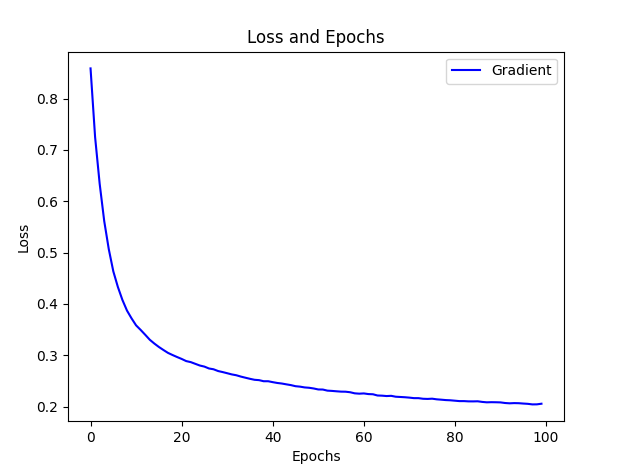
\includegraphics[width=0.8\textwidth]{img1}
\caption{График зависимости функции потерь от числа эпох}
\label{fig:img1}
\end{figure}

\begin{figure}[!htb]
	\centering
	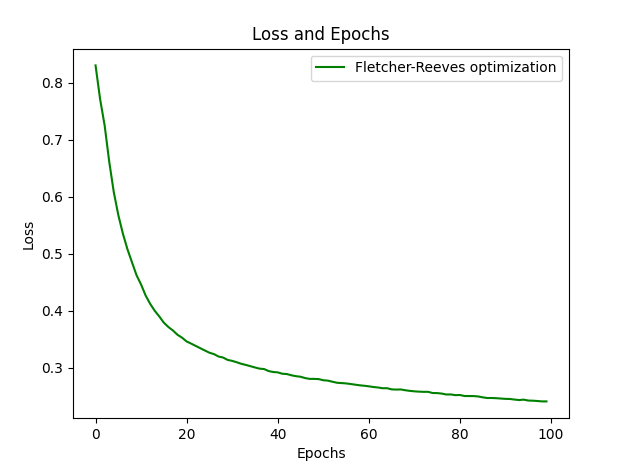
\includegraphics[width=0.8\textwidth]{img2}
\caption{График зависимости функции потерь от числа эпох}
\label{fig:img2}
\end{figure}

\begin{figure}[!htb]
	\centering
	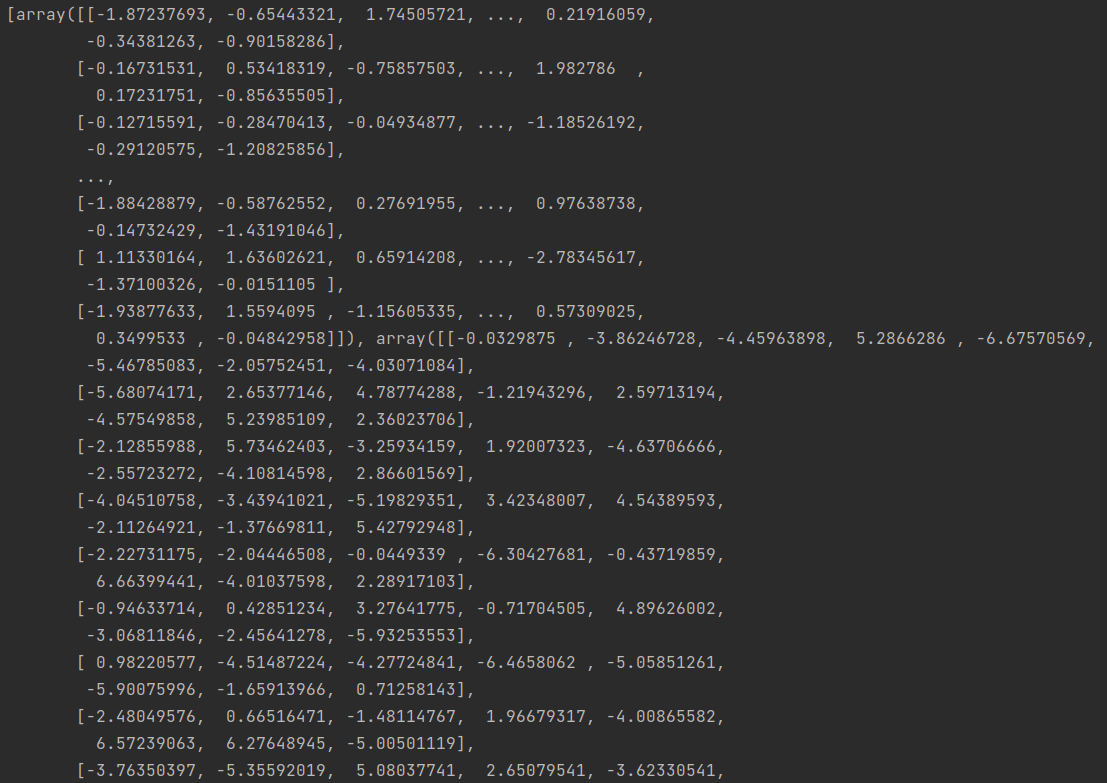
\includegraphics[width=0.8\textwidth]{img3}
\caption{Полученные веса}
\label{fig:img3}
\end{figure}

\begin{figure}[!htb]
	\centering
	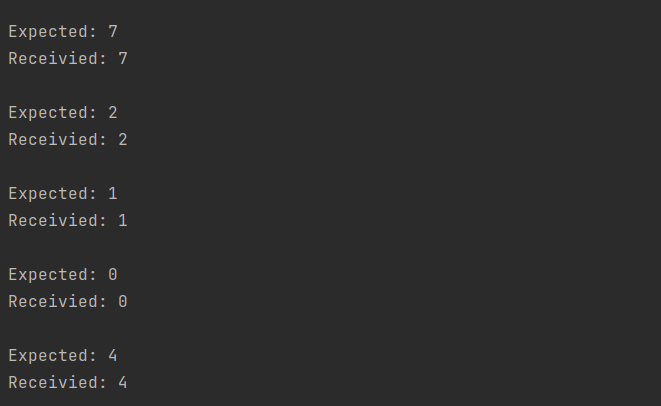
\includegraphics[width=0.8\textwidth]{img4}
\caption{Пример распознавания цифр}
\label{fig:img4}
\end{figure}

\section{Выводы}\label{Sect::conclusion}

В результате выполнения лабораторной работы был реализован многослойный персептрон, были реализованы различные функции активации, функции потерь и оптимизации.

\end{document}
